\chapter{Introduction}
\section{Motivation}
One of several requirements regarding complex life is cell adhesion. If different cells would not stick to each other the only living things would be cells. 
In humans, organs are made of several cells as well as epithels are made of several cells and several layers of cells. This is also the case for the urothelium, which is an epithelium, i.e. a membranous tissue which consists of one or several layers. For the urothelium it is necessary that the cells stick to each other. Otherwise the functions of the urothelium could not be executed and also it would not be able to grow.% If bladder cancer occurs the urothelium also can not function in the way it should do. 

There are two types of tumors. One is the benign and the other one is the malignant tumor \cite{Poplawski2009}. The benign tumor is self limited. Thus, it does not invade surrounding tissues as well as it does not spread into other body parts \cite{Poplawski2009}. The malignant tumor on the other hand is not limited in its growth and is able to invade other body parts \cite{Poplawski2009}. 

Since bladder cancer is one of the most common cancer types among men it is important to understand how and why the cancer is able to grow. \newline
Bladder cancer starts to grow in the urothelium. With the grow and spread, the structure of cells sticking together is changed. In this case, the urothelium is no longer able to completely perform its tasks. In order to understand the urothelium, how and when bladder cancer appears observations of this epithel is necessary. 

To understand the functionalities of organs and epithels, in general organisms, observations are essential. For the urothelium this is already done, as there are a lot of different in vitro experiments about the methodology of the urothelium. After an observation of an epithel or organ is complete, researches are able to predict how the observed organism will react in different situations. To verify these predictions a simulation is necessary. A simulation is an illustration of the reality \cite{REF}, but it can also be used to change reality in a for the research specific way to get more knowledge of the epithel, or an organism in general.

A simulation should always be as simple as possible but also not too simple \cite{REF}. Otherwise the simulation does not represent the reality. 
There are several programs with different algorithms for cell simulation. A popular algorithm is the \ac{GGH} model. This model is popular because it is easy to describe how cells interact with each other and it is possible to define constraints for the volume and surface of each cell. \newline
The program \ac{CC3D} is a simulation program, which uses the \ac{GGH} algorithm in its simulation. In the moduro project we use \ac{CC3D}, and with the program we use the \ac{GGH} algorithm.

The target of the moduro project is to predict under which circumstances bladder cancer occurs and when it is able to grow. Therefore, 16 different morphogenesis models of the urothelium were created. An overview of these models is displayed in table \ref{tbl:16Models} at page \pageref{tbl:16Models}. So far, all 16 models were simulated in 2D for 720 days. The results reveal that some of the models are more realistic and others are less realistic.

Because a cell is a three dimensional organism, a 2D simulation of the urothelium might not give as many aspects as a 3D simulation could do. Thus, the aim of this bachelor thesis is to create a 3D simulation of these 16 different models. With this 3D simulation we hope to receive new insights into the urothelium and how bladder cancer occurs.

\section{Background}
\subsection{Biology of the Urothelium}

\begin{figure}
	\center
	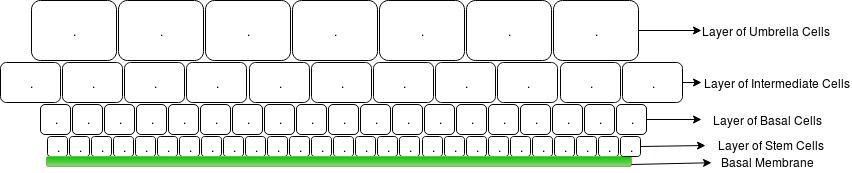
\includegraphics[scale=0.3]{figures/Urothelium.png}
	\caption{A simplified illustration of the urothelium. At the very bottom there is the basal membrane. Above the membrane the stem and basal cells are displayed. The blue cells represent the stem cells, the red cells display the basal cells. Above the layer out of these two cell types, the urothelium contains several layers of intermediate cells. At the top of the urothelium there is an layer of umbrella cells.}
	\label{img:physiology_urothelium}
\end{figure}

Bladder cancer is the 4th most common cancer type in men regarding to everydayhealth.com, where every 36st out of 100.000 men gets it \cite{EveryDayHealth.com}. Bladder cancer usually starts with some cells in the bladder, which grow uncontrolled. From these cells, the tumor can spread further into surrounding areas \cite{Cancer.org}. The most common bladder cancer type is the urothelial carcinoma \cite{Cancer.org}.

The bladder is located in the lower urinary tract and consists of several parts, where the urothelium is one part and coats the bladder \cite{Lazzeri2006}. More specifically, it covers the bladder from the renal pelvis to the proximal urethra \cite{Yamany2014, Birder2005}.

Two important tasks of the bladder are the storage and release of urine. To do so the bladder will extend, during the storage, and then shrink again \cite{Karl-ErikAndersson2004}. One task of the urothelium is to form a distensible barrier \cite{Apodaca2004, Lazzeri2006, PuneetKhandelwal2009, Lewis2000, WRCross2005}, which prevents unregulated exchange of ions, solutes, and toxic metabolites between the bladder and the blood \cite{Apodaca2004, Lazzeri2006, PuneetKhandelwal2009, Lewis2000}. That the urothelium ensures its barrier function, it has to enlarge and downsize its size. This is done by the largest cells of the urothelium, the umbrella cells. Since the umbrella cells are in direct contact with the bladder, it is their task to change size and form during the grow and shrink process of the bladder. Birder described the urothelium as “… a responsive structure capable of detecting physiological and chemical stimuli and releasing a number of signaling mole-cules.” \cite{Birder2005}. Another task of the urothelium is to control the movement and passage of macromolecules, ions, water, toxic metabolites and solutes \cite{Apodaca2004, PuneetKhandelwal2009}. If the urothelium is damaged, it rapidly generates new cells, to ensure full functionality \cite{Apodaca2004, Yamany2014, PuneetKhandelwal2009}.

To receive a better overview the different cell types are explained in the following paragraph. In figure \ref{img:physiology_urothelium} at page \pageref{img:physiology_urothelium} a simplified illustration of the urothelium with its different cell types and cell layers is provided. \newline
The umbrella cells, also called superficial cells, are connected directly with the bladder and have an average diameter of 25 up to \SI{250}{\micro\metre} \cite{Yamany2014, PuneetKhandelwal2009}. 

Below these cells the intermediate cells are located. With an average diameter of 10 up to \SI{20}{\micro\metre} \cite{Yamany2014, PuneetKhandelwal2009}, they are smaller then the umbrella cells. There are at least three and up to five layers of the intermediate cells \cite{REF}. 

The smallest and the most common cells in the urothelium are the basal and stem cells. Those cells have a diameter of up to \SI{10}{\micro\metre} \cite{Lazzeri2006, PuneetKhandelwal2009}. 

The urothelium consits of several layers. In the first layer, there are the basal and stem cells. Above them, there are several layers of intermediate cells. On top of the epithelium there is one layer of umbrella cells.


\subsection{CompuCell3D}
\begin{figure}
	\center
	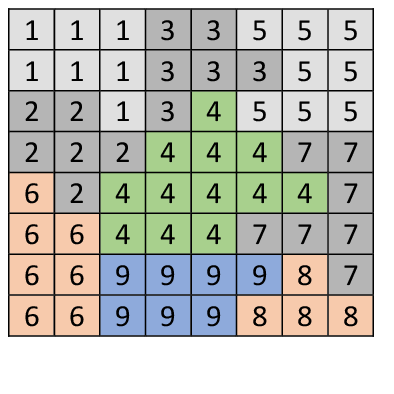
\includegraphics[scale=0.4]{figures/2DSquareLattice.png}
	\caption{A square lattice in 2D. The same digits represent one cell $(\sigma(\vec{i}))$, whereas the different colors represent different cell types $\tau(\sigma)$.}
	\label{img:2DSquareLattice}
\end{figure}
\ac{CC3D} is an open-source program, which provides a simulation environment for multi- or single-cell-based modeling of tissues, organs and organisms \cite{CC3D.org}. To do so, \ac{CC3D} uses the \ac{GGH} model in its simulation. 
CC3D provides the possibility to create programs for the simulation, e.g. cell growth, mitosis, apoptosis or necrosis scripts, in python, C++ or in CC3DML, which is their own Markup Language. With such programs CC3D allows the user to modify the behavior of the simulation for a specific purpose.
CC3D uses the \ac{GGH} approach, explained in section \ref{subsec:Intro_GGH} at page \pageref{subsec:Intro_GGH}. It allows the user to choose between two cell-lattice types, i.e. a presentation of the pixels or voxels of a cell at a specific position in the simulation field. By default it uses a square-lattice of single pixels for each dimension, an example therefore is displayed in figure \ref{img:2DSquareLattice} at page \pageref{img:2DSquareLattice}. There is also the possibility to use a hexagonal-lattice, where the pixels would be hexagons in two dimensions, or rhombic dodecahedrons in three dimensions.
Since the core of a \ac{GGH} simulation is the effective energy \cite{MaciejH.Swat2017}, \ac{CC3D} tries to minimize this effective energy every \ac{MCS}, i.e. a calculation step in the simulation. The basic form for the effective energy is:
\begin{equation}
\mathcal{H}_{boundary} = \sum_{\vec{i},\vec{j}}^{ }{J(\tau(\sigma(\vec{i})),(\tau(\sigma(\vec{j})))(1-\delta(\sigma(\vec{i}),(\sigma(\vec{j})))}
\end{equation}
This equation is a part of the equation of the \ac{GGH} model. The formula of the \ac{GGH} model, and with it this equation, is explained at section \ref{subsec:Intro_GGH} at page \pageref{subsec:Intro_GGH}. \newline
There are two ways to extend this form, it is possible to either add a volume or a surface constraint for each cell. During each \ac{MCS} an index-copy attempt takes place \cite{MaciejH.Swat2017}. Therefore, a pixel is selected, and it is be tried to overwrite a randomly chosen pixel, next to the current pixel, in order to minimize the effective energy. The index copy attempt succeeds and takes place if this index copy attempt decreases the effective energy \cite{MaciejH.Swat2017}. Each \ac{MCS} the program tries to minimize the effective energy with index copy attempts.


\subsection{Glazier Graner Hogeweg Model} \label{subsec:Intro_GGH}
Since there are several formulas and models developed from Glazier and Graner, this subsection briefly describes these models and explains the \ac{CPM} and \ac{GGH} model.\newline
The \ac{GGH} model is widely used in biological simulations, since it provides a good flexibility, extensibility and it is easy to use \cite{Glazier2007}. 
Glazier and Graner developed a model as an extension of the large-q Potts model, which itself is an extension of the Ising Model, and called it first the \ac{EPM}. Nowadays, this model is called \ac{CPM} \cite{Glazier2007, Graner1992, Glazier1993}.
Glazier and Graner extended the \ac{CPM} in a way that also volume constraints are considered for the hamiltonian, see following form:
\begin{equation}\label{eq:H_CPM}
\begin{split}
\mathcal{H}_{CPM} & = \sum_{\vec{i},\vec{j}}^{ }J(\tau(\sigma(\vec{i})),(\tau(\sigma(\vec{j})))(1-\delta(\sigma(\vec{i}),(\sigma(\vec{j}))) \\
		 & + \sum_{\sigma}^{}{\lambda_{vol}((\tau)v(\sigma)-V_{target}(\tau(\sigma)))^2}
\end{split}
\end{equation}
The hamiltonian of equation \ref{eq:H_CPM} describes the effective energy for the extension of the \ac{CPM} model. The first sum describes $J$ of all cells, the adhesion energy between different cells. Therefor, every cell has a specific cell type $\tau(\sigma)$ \cite{Glazier1993, Graner1992}. Each cell is placed onto a lattice with a spin $(\sigma(\vec{i}))$ for every given dimension \cite{Graner1992, Glazier2007}. The adhesion energy between cells is only considered if the kroenecker delta is 0. Thus, the surface energy between cells is considered if $\delta(\sigma, \sigma') = 0$ \cite{Glazier1993, Graner1992, Stott1999, Glazier2007, Chen2007, Cickovski2005}. \newline
With the second sum over all cells the volume of each cell is now considered within the effective energy. The user is now able to set a target volume $V_{target}(\tau(\sigma))$ for each cell, which the cell should have, and a multiplier $\lambda_{vol}$ for the deviation between the current volume $(\tau)v(\sigma)$ and the target volume. During the simulation this deviation is tried to be kept as small as possible for every cell in order to keep the effective energy as small as possible.

Together with Hogeweg they further developed the created extension of the \ac{CPM}. The further developed model is called \ac{GGH} model. The main extension is that the user is now able to add surface area constraints \cite{Graner1992, Glazier1993, Glazier2007} as well as to use a negative boundary energy \cite{Glazier2007}. With the surface constraint the equation for the effective energy of the \ac{GGH} model is: 
\begin{equation}\label{eq:H_GGH}
\begin{split}
\mathcal{H}_{GGH} & = \sum_{\vec{i},\vec{j}}^{ }J(\tau(\sigma(\vec{i})),(\tau(\sigma(\vec{j})))(1-\delta(\sigma(\vec{i}),(\sigma(\vec{j}))) \\
		 & + \sum_{\sigma}^{}{\lambda_{vol}(\tau)v(\sigma)-V_{target}(\tau(\sigma)))^2} \\
		 & + \sum_{\sigma}^{}{\lambda_{sur}(\tau)s(\sigma)-S_{target}(\tau(\sigma)))^2}
\end{split}
\end{equation}
In addition to the hamiltonian of equation \ref{eq:H_CPM} is the surface constraint. It has the same principle as the volume constraint. Thus, the user is able to define a target surface $S_{target}(\tau(\sigma))$ for each cell and a multiplier $\lambda_{sur}$ for the deviation between the target and the actual surface $(\tau)s(\sigma)$ of each cell. Since the volume and surface constraint are included in the effective energy, it should be possible to use these two parts of the effective energy to shape the cells.


Beside the surface constraint the new model allows the user to model (a): cell growth and proliferation (b): mitosis, i.e. cell division (c): fields, forces and diffusion and (d): chemotaxis and haptotaxis \cite{Glazier2007}. \newline
Glazier et. al. describe their model as: 
\begin{quote}
GGH models define biological structure consisting of the configuration of a set of \textit{generalized cells}, each represented on a \textit{cell lattice} as a domain of lattice sites sharing the same cell index [...], a set of \textit{internal cell states} for each cell [...], and a set of \textit{auxiliary fields} ...” \cite{Glazier2007}.
\end{quote}

The \ac{GGH} model has the advantage that “Initial conditions emulating a particular biological configuration rather than random initial conditions.” \cite{Glazier2007} and it has now biologically motivated properties instead of physically motivated properties \cite{Glazier2007}. 


\section{Objective}
The aim of this bachelor thesis is to create a 3D morphogenesis simulation of the urothelium using \ac{CC3D}. Since the simulation models and python program for a 2D simulation are given and the simulation is done by \ac{CC3D} the task is to modify the current application, of the 2D simulation, in a way that this program can be used for a 3D simulation of the different models. \newline
Therefore, some parts of the program have to be modified. Some functionalities have to be invented and developed whereas for other functionalities it is enough to modify these. \newline
The result of this bachelor thesis will be presented with an realistic model of the 2D simulations. This model is chosen from the given models in the 2D simulation. The question how much more time the 3D simulation need than the 2D simulation will be covered in this thesis as well. If it is possible to provide a calculation of how much more effort a simulation in three dimensions need it will be included, otherwise an estimation of the more effort is presented.


\section{Outline}
In this chapter the knowledge to understand this bachelor thesis is provided. The next chapter provides the status at which the project was at the beginning of this bachelor thesis. Once the basic knowledge and the state of the art are explained, necessary modifications of the program are revealed. After these modifications are presented, the result of this bachelor thesis is shown. In the last section of this thesis, this work is discussed from different points of view and the conclusion out of this work is presented.